% mn2esample.tex
%
% v2.1 released 22nd May 2002 (G. Hutton)
%
% The mnsample.tex file has been amended to highlight
% the proper use of LaTeX2e code with the class file
% and using natbib cross-referencing. These changes
% do not reflect the original paper by A. V. Raveendran.
%
% Previous versions of this sample document were
% compatible with the LaTeX 2.09 style file mn.sty
% v1.2 released 5th September 1994 (M. Reed)
% v1.1 released 18th July 1994
% v1.0 released 28th January 1994

\documentclass[useAMS,usenatbib]{mn2e}
\usepackage{graphicx}
\usepackage{journals}
\usepackage{amsmath}
\def\5{\footnotesize V\normalsize}
\def\4{\footnotesize IV\normalsize}
\def\3{\footnotesize III\normalsize}
\def\2{\footnotesize II\normalsize}
\def\1{\footnotesize I\normalsize}
\def\lam{$\lambda$}
\def\kms{$\mbox{km s}^{-1}$}
\def\p{$\phantom{:}$}
\def\a{$\phantom{^\ast}$}
\def\v{$\phantom{^{l}}$}
\def\pp{$\phantom{-}$}
\def\o{$\phantom{0}$}
\def\vr{$v_{\rm r}$}


% If your system does not have the AMS fonts version 2.0 installed, then
% remove the useAMS option.
%
% useAMS allows you to obtain upright Greek characters.
% e.g. \umu, \upi etc.  See the section on "Upright Greek characters" in
% this guide for further information.
%
% If you are using AMS 2.0 fonts, bold math letters/symbols are available
% at a larger range of sizes for NFSS release 1 and 2 (using \boldmath or
% preferably \bmath).
%
% The usenatbib command allows the use of Patrick Daly's natbib.sty for
% cross-referencing.
%
% If you wish to typeset the paper in Times font (if you do not have the
% PostScript Type 1 Computer Modern fonts you will need to do this to get
% smoother fonts in a PDF file) then uncomment the next line
% \usepackage{Times}

%%%%% AUTHORS - PLACE YOUR OWN MACROS HERE %%%%%


%%%%%%%%%%%%%%%%%%%%%%%%%%%%%%%%%%%%%%%%%%%%%%%%

\title[Red Supergiants as Cosmic Abundance Probes: NGC\,2100]{Red Supergiants as Cosmic Abundance Probes: NGC\,2100}
\author[L. R. Patrick et al.]{L. R. Patrick$^{1}$\thanks{E-mail: lrp@roe.ac.uk}, C. J. Evans$^{1, 2}$, B. Davies$^{3}$, et al.\\
$^{1}$Institute for Astronomy, University of Edinburgh, Royal Observatory Edinburgh, Blackford Hill, Edinburgh EH9 3HJ, UK\\
$^{2}$UK Astronomy Technology Centre, Royal Observatory Edinburgh, Blackford Hill, Edinburgh EH9 3HJ, UK\\
$^{3}$Astrophysics Research Institute, Liverpool John Moores University, Liverpool Science Park ic2, 146 Brownlow Hill, Liverpool L3 5RF, UK
}

% \author[A. V. Raveendran and A. N. Other]{A. V. Raveendran$^{1}$\thanks{E-mail:
% email@address (AVR); otheremail@otheraddress (ANO)} and A. N.
% Other$^{2}$\footnotemark[1]\thanks{This file has been amended to
% highlight the proper use of \LaTeXe\ code with the class file.
% These changes are for illustrative purposes and do not reflect the
% original paper by A. V. Raveendran.}\\
% $^{1}$Indian Institute of Astrophysics, Bangalore 560034, India\\
% $^{2}$Building, Institute, Street Address, City, Code, Country}
\begin{document}

\date{Accepted  Received 1; in original form}

\pagerange{\pageref{firstpage}--\pageref{lastpage}} \pubyear{2015}

\maketitle

\label{firstpage}

\begin{abstract}
We have obtained KMOS spectroscopy for 17 red supergiant stars in the Large Magellanic Cloud (LMC) massive star cluster NGC\,2100.
Stellar parameters have been derived and are shown to ... compared to previous results.\\
Radial velocities are estimated for the targets ... .\\


\end{abstract}

\begin{keywords}
Red Supegiants: stars.
\end{keywords}

\section{Introduction} % (fold)
\label{sec:introduction}

Something great about the LMC and how NGC\,2100 fits into the mix.
NGC\,2100 is a young massive star cluster located on the near edge of the LMC, near the 30 Dor region.
There have been many studies which have identified a large number of RSGs within the cluster.
This is the first quantitative estimate of their metallicities.

Some NGC\,2100 stats:\\
Age: 20\,Myr~\citep{2015A&A...575A..62N} \\
Mass: $4.36\times10^{4}$~\citep{2005ApJS..161..304M}\\
R$_{core}$ (pc): 3.03/0.99~\citep{2005ApJS..161..304M}\\
Z: $log0.007/Z_{\odot} = -0.34$~\citep{2015A&A...575A..62N}\\
V$_{esc}$ (\kms): 7.9~\citep{2005ApJS..161..304M}\\



Questions we would like to answer in this paper:\\
Are the known RSGs in this region genuine cluster members and if so what does their velocity dispersion look like?\\

How does the metallicity of these objects relate the to that in the nearby 30 Dor region and other RSGs within this galaxy?


% section introduction (end)

\section{Observations and Data Reduction} % (fold)
\label{sec:observations}
\subsection{Target Selection} % (fold)
\label{sub:target_selection}

\begin{itemize}
  \item How were these targets selected?
\end{itemize}

\begin{figure}
 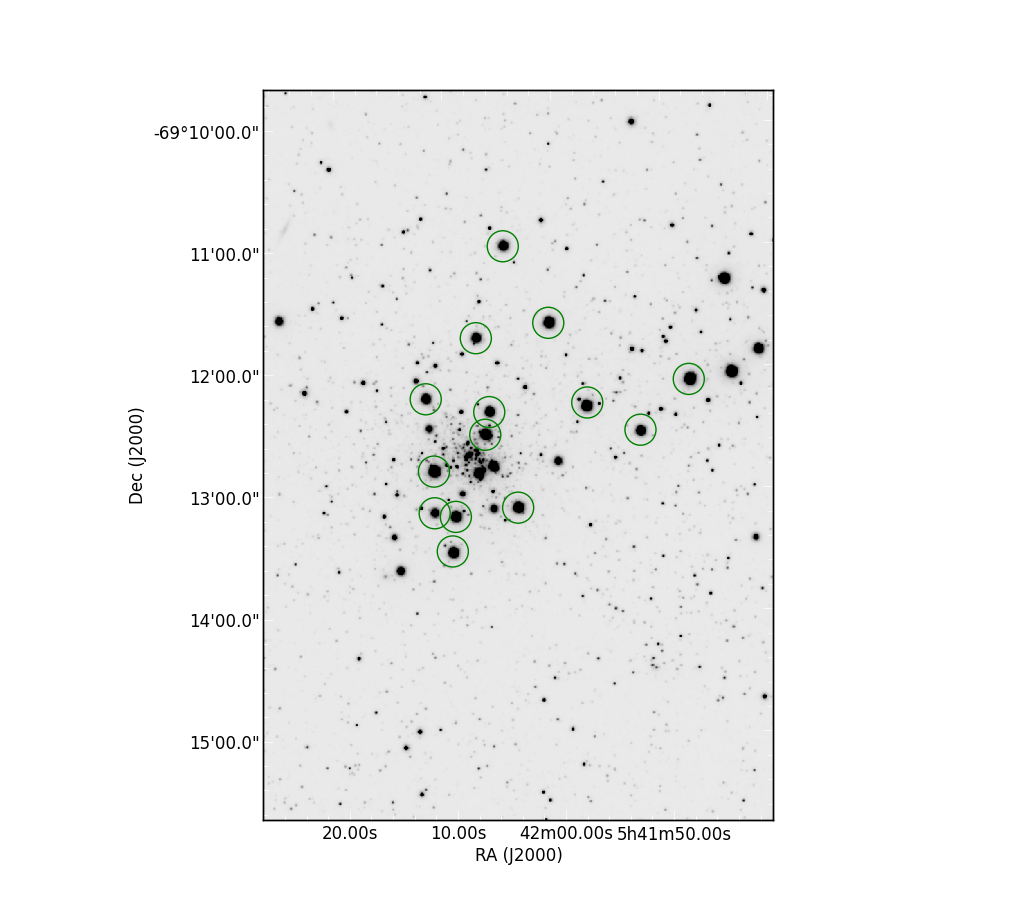
\includegraphics[width=9.0cm]{NGC2100-targets}
 \caption{Positions of the NGC\,2100 KMOS targets overlaid on a VISTA $J$-band image.
\label{fig:targets}
          }
\end{figure}

% subsection target_selection (end)
\subsection{KMOS Observations} % (fold)
\label{sub:kmos_observations}

% subsection kmos_observations (end)
These observations form part of the KMOS Gaurenteed Time Observing (PI: Evans) and were conducted in March 2015.
The observations consist of $8\times10$\,s exposures taken with the YJ grating with sky offset exposures (S) interleaved between the object (O) exposures in an O,~S,~O observing pattern.
In addition, a standard set of KMOS calibration frames were also obtained as well as telluric standard frames using HIPXXX as the telluric standard star.
Seeing conditions were stable at 1.0\,arcseconds for the course of the observations.

The KMOS/esorex standard routines~\citep[SPARK;]{2013A&A...558A..56D} were used to calibration and reconstruct the data cubes.
Telluric correction was performed using the 24-arm telluric correction routine (described in detail in ~\cite{2015ApJ...803...14P}).
Briefly, corrections to the standard telluric recipe are put in place to correct for slight differences in wavelength calibration between the telluric and science spectra.
This is implemented using an itertive cross-correlation approach.
Additionally, differences in the strength of the telluric features are corrected by apply a simple scaling.
Once these corrections are in place, the scicence spectra are divided by the appropriate telluric spectrum for that particular IFU.


\begin{table*}
\caption{
        Summary of VLT-KMOS targets in NGC\,6822.\label{tb:obs-params}
        }
\scriptsize
\begin{center}
\begin{tabular}{lrcccccccccl}
 \hline
 \hline
ID & S/N & $\alpha$ (J2000) & $\delta$ (J2000) & $B$ & $V$ & $I$ & $J$ & $H$ & $K_{\rm s}$ & RV (\kms) & Notes \\
 \hline
0207-0134568 & 318 & 05:41:47.873 & -69:12:05.959 & 16.488 & 13.749 &  9.769 &  9.525 &  8.603 & 8.200 & 233.989\\
0207-0134683 & 198 & 05:41:52.430 & -69:12:30.410 & 16.430 & 14.267 & 11.970 & 10.413 &  9.526 & 9.155 & 213.781\\
0207-0134811 & 202 & 05:41:57.286 & -69:12:16.480 & 14.074 & 13.019 & 11.170 &  9.811 &  9.036 & 8.738 & 253.005\\
0207-0134979 & 252 & 05:42:03.877 & -69:13:07.410 & 15.624 & 13.579 & 11.410 &  9.839 &  8.996 & 8.740 & 246.637\\
0207-0135059 & 196 & 05:42:06.348 & -69:12:20.150 & 00.000 & 00.000 & 11.810 & 10.371 &  9.480 & 9.159 & 248.928\\
0207-0135069 & 256 & 05:42:06.764 & -69:12:31.245 & 15.643 & 13.675 & 11.390 &  9.977 &  9.150 & 8.807 & 245.703\\
0207-0135150 & 240 & 05:42:09.647 & -69:13:11.263 & 15.367 & 13.383 & 11.370 &  9.976 &  9.136 & 8.841 & 247.856\\
0207-0135162 & 250 & 05:42:10.001 & -69:13:28.210 & 16.060 & 13.827 & 11.580 & 10.021 &  9.150 & 8.823 & 246.984\\
0207-0135205 & 304 & 05:42:11.574 & -69:12:48.770 & 16.327 & 14.033 & 11.450 &  9.557 &  8.617 & 8.264 & 245.22\\
0207-0135206 & 151 & 05:42:11.592 & -69:13:09.257 & 16.165 & 14.272 & 12.340 & 10.943 & 10.090 & 9.788 & 232.663\\
0207-0135220 & 195 & 05:42:12.182 & -69:12:13.144 & 15.483 & 13.606 & 11.750 & 10.440 &  9.622 & 9.335 & 290.345\\
0208-0135292 & 262 & 05:42:00.722 & -69:11:36.925 & 15.579 & 13.674 &  9.421 &  9.900 &  9.017 & 8.683 & 246.551\\
0208-0135383 & 211 & 05:42:04.762 & -69:10:58.816 & 15.550 & 13.800 & 12.770 & 10.319 &  9.427 & 9.159 & 252.045\\
0208-0135446 & 201 & 05:42:07.435 & -69:11:43.692 & 15.531 & 13.661 & 11.780 & 10.482 &  9.610 & 9.351 & 271.205\\
\hline
\end{tabular}
\end{center}
{Photometric data taken from the SIMBAD database. Typical errors on photometric data:
0.026, 0.014, 0.04, 0.024, 0.026, 0.022 respectively.
Near-IR data taken from 2MASS.}
\end{table*}

\subsection{Data Reduction} % (fold)
\label{sub:data_reduction}

% subsection data_reduction (end)
% section observations (end)

\section{Radial velocities} % (fold)
\label{sec:radial_velocities}
Radial velocities are estimated using an iterative cross-correlation method.
To ensure the KMOS spectra are at rest wavelength, the observed spectra are first cross-correlated against a model telluric spectrum, taken from the ISSAC web-pages, which is known to be at a much higher resolution than that of the observations.
This cross-correlation is performed in the $1.15-1.17\,\mu$m region as this is where the telluric features dominate.

Once the observed spectra are at rest wavelength, an initial guess of the radial velocity is estimated by cross-correlating the science spectra with an appropriate synthetic RSG spectrum in the $1.17-1.21\,\mu$m region.
This wavelength regime is selected based on the dominance of atomic features in the RSG spectrum at these wavelengths.
To increase reliability, this initial guess is improved upon by using five carefully selected groups of stellar absorption lines centred on some of the strongest atomic features in this region.
These lines and regions are selected based on their reliability and are known to be not affected by telluric absorption.
Figure~\ref{fig:rv-regions} illustrates which features have been used for the analysis.

Radial velocities are independently calculatedfor each of region by means of iterative cross-correlation.
This results in five estimates of the radial velocity for each star which are then compared and any region which produces a radial velocity which is an obvious outlier to the distribution is rejected.
The final radial velocity for each star is the mean of the distribution resulting from the (non-rejected) regions.
The error on this mean is calculated by taking the standard deviation of the data, normalised by the number of regions used ($err~=~\sigma/N_{regions}$).
This method is shown to work well for KMOS spectra~\citep{2015ApJ...798...23L,2015ApJ...803...14P}.

Figure~\ref{fig:rvs} shows the radial velocities for all targets as a function of distance from the centre of the cluster, shown alongside the systemic radial velocity of the LMC (green dashed line; see section~\ref{sec:discussion} for a discussion on this).
% Here the cluster centre is defined ...

An upper limit to the line-of-sight velocity dispersion can calculated using the equations,
\begin{equation}
  \mu = \frac{1}{\sum_{i} 1/\sigma_{i}^{2}} \sum_{i} \frac{RV_{i}}{\sigma_{i}},
\end{equation}

\begin{equation}
Var = \frac{1}{\sum_{i}1/\sigma_{i}^{2}} \sum_{i}\frac{(RV_{i} - \mu)^{2}}{\sigma_{i}^{2}},
\end{equation}

\begin{equation}
  \sigma_{1D} = \sqrt{Var \frac{N}{N - 1}}
\end{equation}

\noindent where $\sigma_{i}$ is the uncertainty on the radial velocity measurement $RV_{i}$ and $N$ is the number of stars in the sample~\citep[and references therin]{2012A&A...546A..73H}.

Using $\sigma_{1D}$ as an upper limit on the velocity distribution, one can calculate the dynamical/virial mass of the cluster using the equation,

\begin{equation}
  M_{vir} = \frac{\eta\sigma_{1D}^{2}r_{eff}}{G}
\end{equation}

\noindent where $M_{vir}$ is the virial mass, $\eta~=6r_{vir}/r_{eff}~=~9.75$ providing the density profile of the cluster is sufficently steep~\citep{2010ARA&A..48..431P}.
However, NGC\,2100 has a relatively shallow density profile ($\gamma~=~2.3$) which means $\eta>9.75$ therefore the estimate of $M_{vir}$ is knowingly an overestimate.
Using this wq

\begin{figure*}
 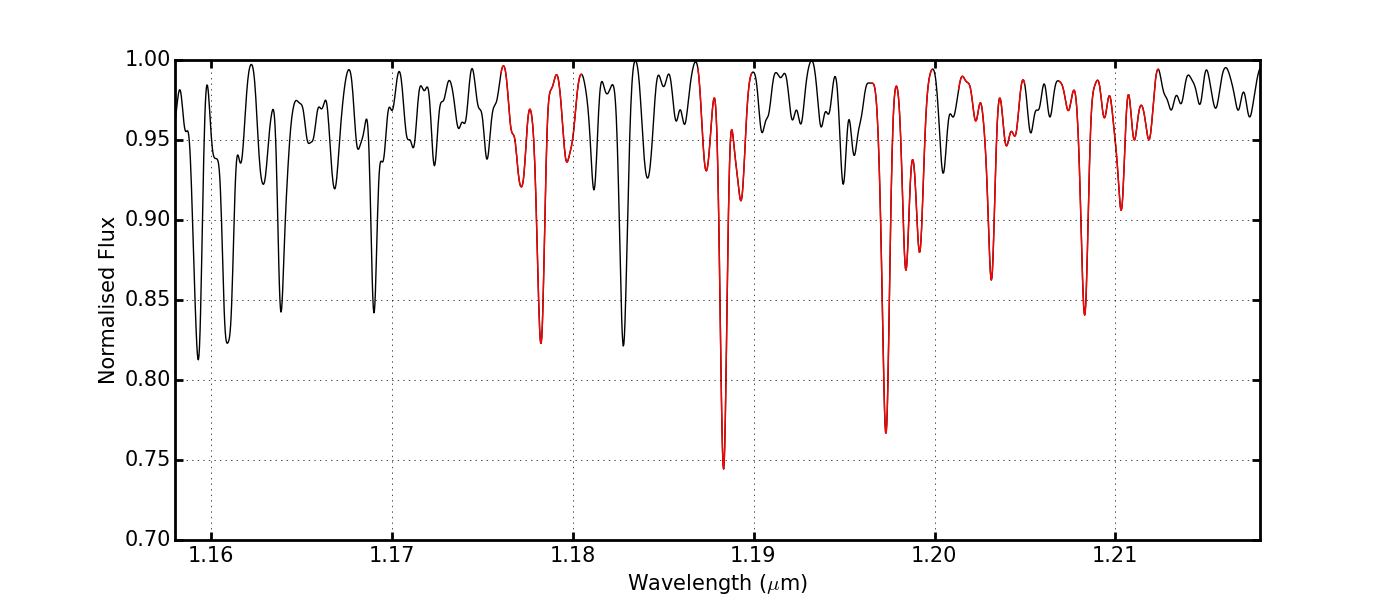
\includegraphics[width=18.0cm]{NGC2100-rv-regions}
 \caption{Sythetic RSG spectrum used calcualte the radial velocities for programme stars.
 Red regions illustrate regions where a cross-correlation is performed between the observed spectra and this synthetic spectrum.
 These regions provide consistent results with an average dispersion between the five regions of of 2.3\,\kms.
\label{fig:rv-regions}
          }
\end{figure*}


\begin{figure}
 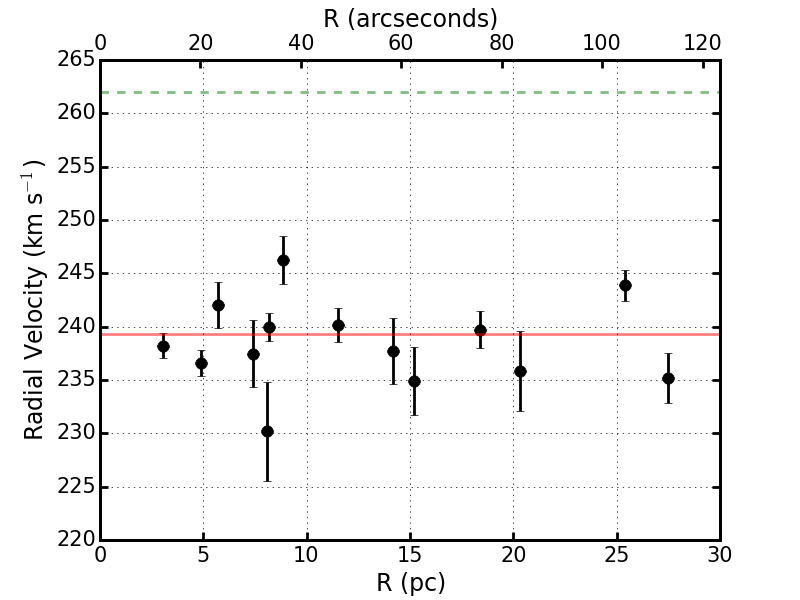
\includegraphics[width=9.0cm]{NGC2100-rv-v4}
 \caption{Radial velocities of KMOS targets shown as a function of distance from the cluster centre.
 Green dashed line shows the LMC systemtic veloctiy~\citep[$262.2\pm3.4$\,\kms;][]{2012AJ....144....4M}
 and the solid red line shows the mean of the sample ($248\pm17\,$\kms).
\label{fig:rvs}
          }
\end{figure}
% section radial_velocities (end)

\section{Stellar parameters} % (fold)
\label{sec:stellar_parameters}

Stellar paramaeters are estimated using the J-band analysis technique descibred initially in~\cite{2010MNRAS.407.1203D}
and tested rigorously in~\cite{2014ApJ...788...58G} and~\cite{2015ApJ...806...21D}.
These studies show that using a narrow spectral window within the $J$-band one can accurately derive global metallicitiy ([Z]) to within
$\pm0.2\,dex$ at the resolution of KMOS observations with S/N~$\ge~100$.
The ranges of each parameter for the grid of model spectra are listed in table~\ref{tb:mod_range}.

\begin{itemize}
  \item Stellar parameters for all targets are listed in table~\ref{tb:stellar-params}.
  \item How do we know these parameters are ligit?
  \item Compare to Ben's implemenation
  \item find some previous studies of young stars in this cluster
\end{itemize}

Stellar parameters have been derived using the J-band analysis technique described in~\cite{2010MNRAS.407.1203D}.
This however, includes the affects of magnesium in the analysis by using two strong magnesium absorption lines which are known to be affected strongly by non-LTE effects~\citep{2015ApJ...804..113B}.
In order to use these lines~\cite{2015ApJ...804..113B} calcualte non-LTE corrections for these magnesium lines.
This also allows one to derive a metallicitiy based solely on the $\alpha$ elements allowing one to derive the [$\alpha$/Fe] ratio.
This is the first time which this technique has been used to estimate this parameter.
The parameters fitted are defined in table

\begin{itemize}
  \item Comparisons to previous studies of young stars in this region
  \item Compare to LMC-wdie studies of young stars
  \item How does it compare to Davies et al. 2015? Do I also see this slightly high Z?
  \item Is this cluster special?
  \item We know it is young and massive in one of the most vigously star forming regions in the local universe
\end{itemize}


\begin{figure*}
 %\vspace{302pt}
 \begin{center}
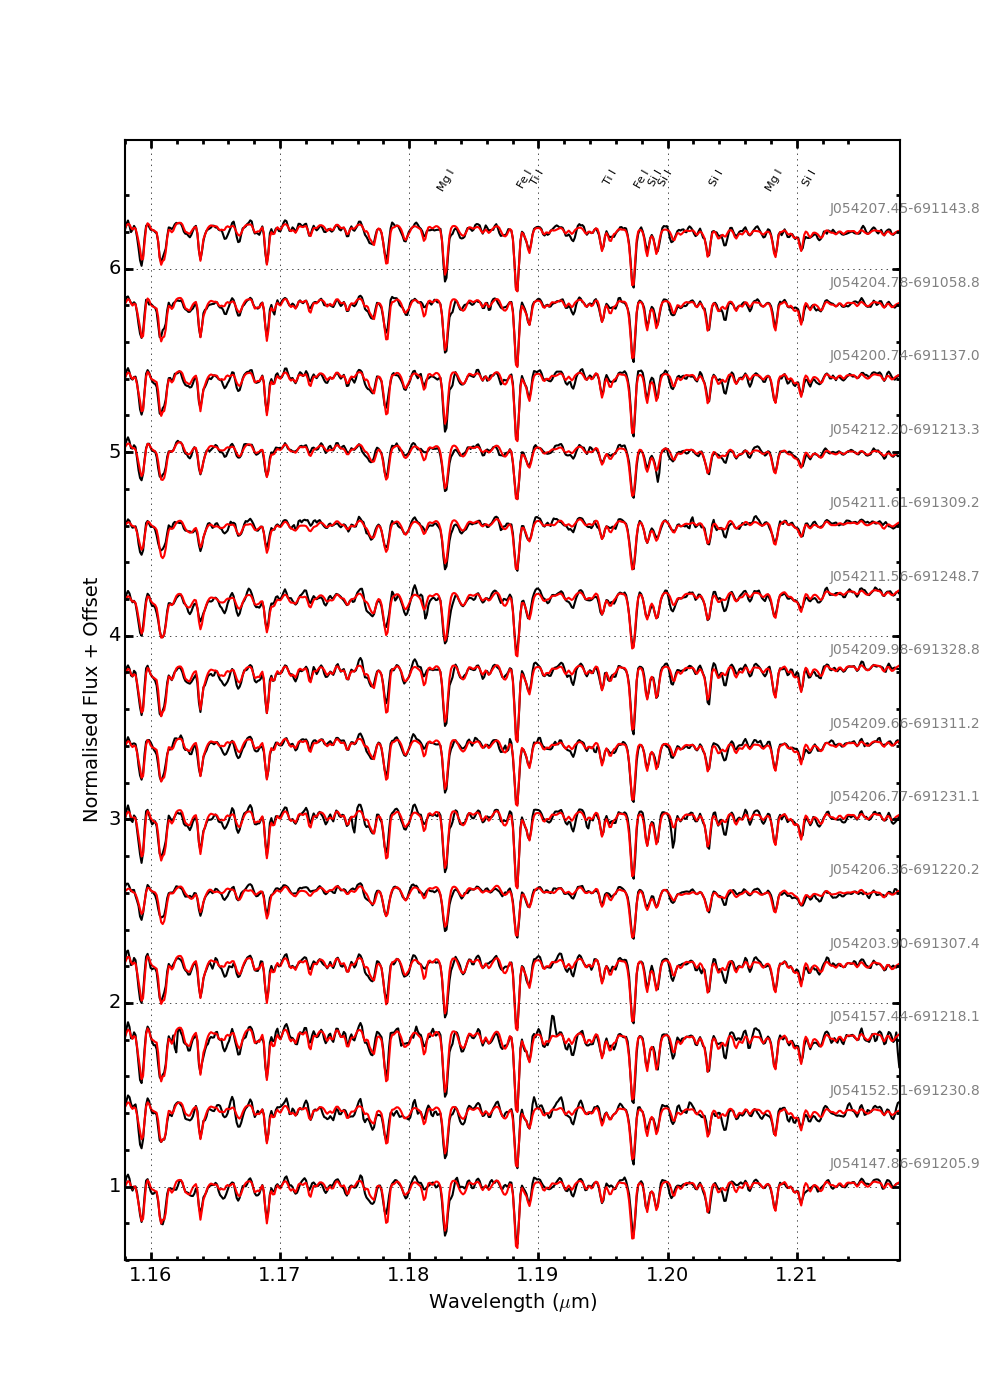
\includegraphics[width=16cm]{NGC2100-model-fits}
\caption{KMOS spectra of the NGC\,6822 RSGs and their associated best-fit model spectra
(black and red lines, respectively).
The lines used for the analysis from left-to-right by species are:
Fe\,I$\lambda\lambda$1.188285,
1.197305,
Si\,I$\lambda\lambda$1.198419,
1.199157,
1.203151,
1.210353,
Ti\,I$\lambda\lambda$1.189289,
1.194954.
The two strong Mg\,I lines are also labelled, but are not used in the fits
(see Section~\ref{sec:results}).
         }
\label{fig:model_fits}
\end{center}
\end{figure*}




\begin{figure}
 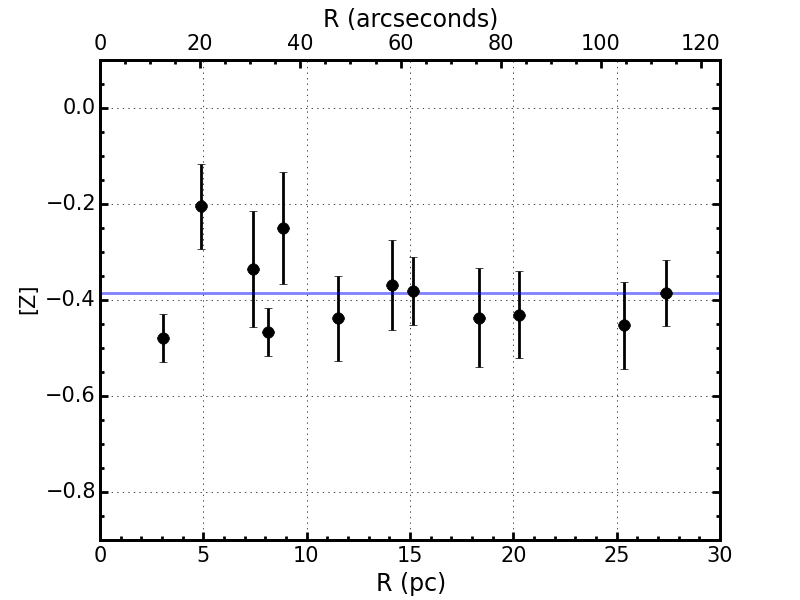
\includegraphics[width=9.0cm]{NGC2100-ZvsR}
 \caption{Estimated metallicities shown against distance from the centre of the cluster.
\label{fig:ZvsR}
          }
\end{figure}

\begin{table}
\caption{
Model grid used for analysis.
\textbf{This needs to be updated for new grids!}\label{tb:mod_range}
         }
\scriptsize
\begin{center}
\begin{tabular}{lccc}
 \hline
 \hline
  Model Parameter & Min. & Max. & Step size \\
 \hline
T$_{eff}$ (K)        & 3400 & 4000 & 100 \\
                     & 4000 & 4400 & 200 \\
$[$Z$]$ (dex)   & $-$1.50 & 1.00  & 0.25\\
log\,$g$ (cgs)  & $-$1.0\o & 1.0\o & 0.5\o \\
 $\xi$ (\kms)  & \pp1.0\o & 6.0\o & 1.0\o\\
 \hline
\end{tabular}
\end{center}
\end{table}

\begin{table*}
\begin{center}
\caption{
Fit parameters for NGC\,2100 KMOS targets
\label{tb:stellar-params}
         }
\scriptsize
\begin{tabular}{lc cccc}
 \hline
 \hline
  Target  & IFU & $\xi$ (\kms) & [Z] & log\,$g$ & T$_{eff}$ (K)\\
  \hline
0207-0134568 & \# & 4.0 $\pm$ 0.3 & -0.40 $\pm$ 0.15 &  0.4  $\pm$ 0.3  & 3890 $\pm$ 70\\
0207-0134683 & \# & 3.5 $\pm$ 0.2 & -0.79 $\pm$ 0.09 & -0.5  $\pm$ 0.11 & 3800 $\pm$ 40\\
0207-0134811 & \# & 5.0 $\pm$ 0.2 & -0.30 $\pm$ 0.14 & -0.10 $\pm$ 0.4  & 3980 $\pm$ 60\\
0207-0134979 & \# & 4.3 $\pm$ 0.3 & -0.48 $\pm$ 0.15 & -0.10 $\pm$ 0.4  & 3840 $\pm$ 70\\
0207-0135059 & \# & 3.0 $\pm$ 0.6 & -0.68 $\pm$ 0.35 & -0.13 $\pm$ 0.4  & 3720 $\pm$ 80\\
0207-0135069 & \# & 4.7 $\pm$ 0.2 & -0.63 $\pm$ 0.13 & -0.7  $\pm$ 0.28 & 3700 $\pm$ 40\\
0207-0135150 & \# & 4.0 $\pm$ 0.2 & -0.52 $\pm$ 0.14 & -0.10 $\pm$ 0.4  & 3720 $\pm$ 70\\
0207-0135162 & \# & 5.0 $\pm$ 0.0 & -0.96 $\pm$ 0.0  & -0.5  $\pm$ 0.0  & 3520 $\pm$ 00\\
0207-0135205 & \# & 3.8 $\pm$ 0.3 & -0.61 $\pm$ 0.19 & -0.5  $\pm$ 0.5  & 3600 $\pm$ 70\\
0207-0135206 & \# & 3.13$\pm$ 0.4 & -0.57 $\pm$ 0.31 &  0.13 $\pm$ 0.4  & 3630 $\pm$ 70\\
0207-0135220 & \# & 3.3 $\pm$ 0.3 & -0.54 $\pm$ 0.17 &  0.3  $\pm$ 0.5  & 3940 $\pm$ 80\\
0208-0135292 & \# & 4.0 $\pm$ 0.2 & -0.74 $\pm$ 0.16 & -0.6  $\pm$ 0.4  & 3710 $\pm$ 70\\
0208-0135383 & \# & 4.18$\pm$ 0.3 & -0.62 $\pm$ 0.17 & -0.10 $\pm$ 0.4  & 3690 $\pm$ 60\\
0208-0135446 & \# & 4.05$\pm$ 0.3 & -0.49 $\pm$ 0.18 & -0.05 $\pm$ 0.5  & 3730 $\pm$ 70\\

  \hline
  \end{tabular}
  \end{center}
\end{table*}

% section stellar_parameters (end)

\section{Discussion} % (fold)
\label{sec:discussion}

\begin{itemize}
  \item What does this mean for stellar evolution models?
  \item Can we say anything interesting about what $\alpha$ should be?
  \item Will we have $\alpha$ at all?
  \item Do these Teff's fit into the picture?
  \item Can we believe the Z's?
  \item Can we say anything about an age spread? (Niederhofer et al. 2015)
  \item e.g. is the distribution of masses what we would expect from a single stellar population?
  \item
\end{itemize}

\begin{figure}
 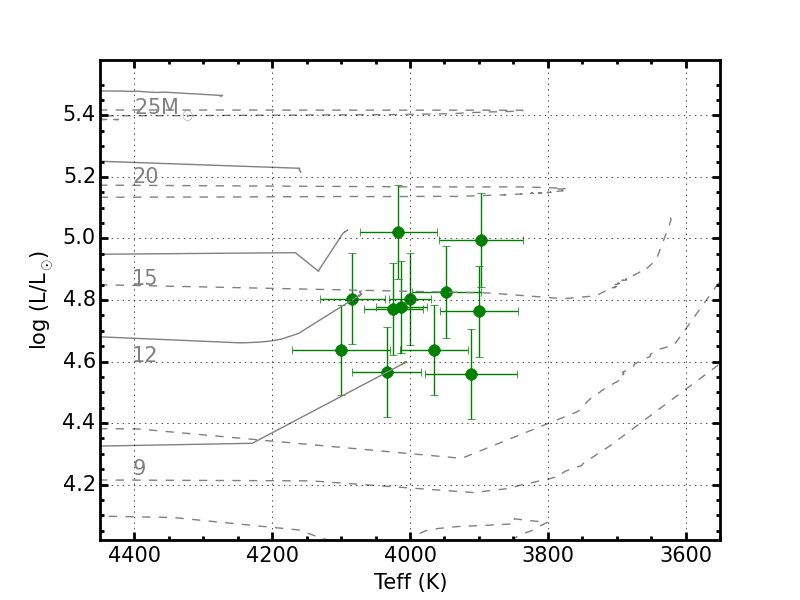
\includegraphics[width=9.0cm]{NGC2100-HRD}
 \caption{Estimated metallicities shown against distance from the centre of the cluster.
\label{fig:HRD}
          }
\end{figure}

\begin{figure}
 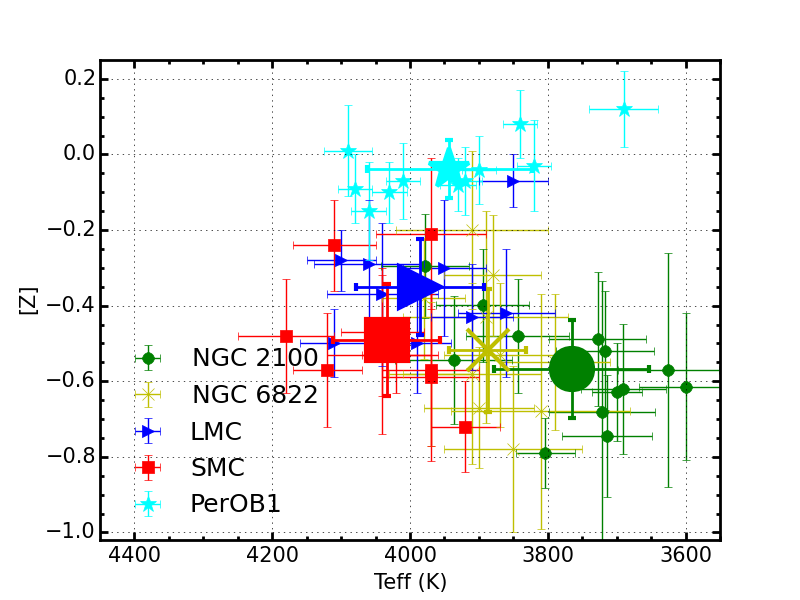
\includegraphics[width=9.0cm]{NGC2100-TeffvsZ}
 \caption{Estimated metallicities shown against estimated effective temperature.
\label{fig:TeffvsZ}
          }
\end{figure}

% section discussion (end)

\section{Conclusions} % (fold)
\label{sec:conclusions}

% section conclusions (end)
\section*{Acknowledgments}

...
\bibliography{journals}

\begin{thebibliography}{99}

\bibitem[Bergemann et al.(2012)]{2012ApJ...751..156B} Bergemann, M.,
Kudritzki, R.-P., Plez, B., et al.\ 2012, \apj, 751, 156

\bibitem[Bergemann et al.(2013)]{2013ApJ...764..115B} Bergemann, M.,
Kudritzki, R.-P., W{\"u}rl, M., et al.\ 2013, \apj, 764, 115

\bibitem[Bergemann et al.(2015)]{2015ApJ...804..113B} Bergemann, M.,
Kudritzki, R.-P., Gazak, Z., Davies, B., \& Plez, B.\ 2015, \apj, 804, 113

\bibitem[Davies et al.(2010)]{2010MNRAS.407.1203D} Davies, B., Kudritzki,
R.-P., \& Figer, D.~F.\ 2010, \mnras, 407, 1203

\bibitem[Davies et al.(2015)]{2015ApJ...806...21D} Davies, B., Kudritzki,
R.-P., Gazak, Z., et al.\ 2015, \apj, 806, 21

\bibitem[Davies et
al.(2013)]{2013A&A...558A..56D} Davies, R.~I., Agudo Berbel, A., Wiezorrek, E., et al.\ 2013, \aap, 558, A56

\bibitem[Gazak et al.(2014)]{2014ApJ...788...58G} Gazak, J.~Z., Davies, B.,
Kudritzki, R., Bergemann, M., \& Plez, B.\ 2014, \apj, 788, 58

\bibitem[Gazak et al.(2014)]{2014ApJ...787..142G} Gazak, J.~Z., Davies, B.,
Bastian, N., et al.\ 2014, \apj, 787, 142

\bibitem[H{\'e}nault-Brunet et
al.(2012)]{2012A&A...546A..73H} H{\'e}nault-Brunet, V., Evans, C.~J., Sana, H., et al.\ 2012, \aap, 546, A73

\bibitem[Lapenna et al.(2015)]{2015ApJ...798...23L} Lapenna, E., Origlia,
L., Mucciarelli, A., et al.\ 2015, \apj, 798, 23

\bibitem[McConnachie(2012)]{2012AJ....144....4M} McConnachie, A.~W.\ 2012,
\aj, 144, 4

\bibitem[McLaughlin
\& van der Marel(2005)]{2005ApJS..161..304M} McLaughlin, D.~E., \& van der Marel, R.~P.\ 2005, \apjs, 161, 304

\bibitem[Niederhofer et
al.(2015)]{2015A&A...575A..62N} Niederhofer, F., Hilker, M., Bastian, N., \& Silva-Villa, E.\ 2015, \aap, 575, A62

\bibitem[Patrick et al.(2015)]{2015ApJ...803...14P} Patrick, L.~R., Evans,
C.~J., Davies, B., et al.\ 2015, \apj, 803, 14

\bibitem[Portegies Zwart et
al.(2010)]{2010ARA&A..48..431P} Portegies Zwart, S.~F., McMillan, S.~L.~W., \& Gieles, M.\ 2010, \araa, 48, 431

\end{thebibliography}
\label{lastpage}

\end{document}
